\chapter{Diseño e Implementación} % Main chapter title

\label{Chapter3} % Change X to a consecutive number; for referencing this chapter elsewhere, use \ref{ChapterX}
\definecolor{mygreen}{rgb}{0,0.6,0}
\definecolor{mygray}{rgb}{0.5,0.5,0.5}
\definecolor{mymauve}{rgb}{0.58,0,0.82}

\lstset{ %
  backgroundcolor=\color{white},   % choose the background color; you must add \usepackage{color} or \usepackage{xcolor}
  basicstyle=\footnotesize,        % the size of the fonts that are used for the code
  breakatwhitespace=false,         % sets if automatic breaks should only happen at whitespace
  breaklines=true,                 % sets automatic line breaking
  captionpos=b,                    % sets the caption-position to bottom
  commentstyle=\color{mygreen},    % comment style
  deletekeywords={...},            % if you want to delete keywords from the given language
  %escapeinside={\%*}{*)},          % if you want to add LaTeX within your code
  %extendedchars=true,              % lets you use non-ASCII characters; for 8-bits encodings only, does not work with UTF-8
  %frame=single,	                   % adds a frame around the code
  keepspaces=true,                 % keeps spaces in text, useful for keeping indentation of code (possibly needs columns=flexible)
  keywordstyle=\color{blue},       % keyword style
  language=[ANSI]C,					% the language of the code
  %otherkeywords={*,...},           % if you want to add more keywords to the set
  numbers=left,                    % where to put the line-numbers; possible values are (none, left, right)
  numbersep=5pt,                   % how far the line-numbers are from the code
  numberstyle=\tiny\color{mygray}, % the style that is used for the line-numbers
  rulecolor=\color{black},         % if not set, the frame-color may be changed on line-breaks within not-black text (e.g. comments (green here))
  showspaces=false,                % show spaces everywhere adding particular underscores; it overrides 'showstringspaces'
  showstringspaces=false,          % underline spaces within strings only
  showtabs=false,                  % show tabs within strings adding particular underscores
  stepnumber=1,                    % the step between two line-numbers. If it's 1, each line will be numbered
  stringstyle=\color{mymauve},     % string literal style
  tabsize=2,	                   % sets default tabsize to 2 spaces
  title=\lstname,                   % show the filename of files included with \lstinputlisting; also try caption instead of title
  morecomment=[s]{/*}{*/}%
}

En este capítulo se presenta la arquitectura del \textit{firmware} y el patrón de diseño usado para los módulos del sistema. Asimismo, se detallan aspectos funcionales de cada módulo y se fundamentan las elecciones de los distintos componentes de hardware utilizados.

El código fuente asociado puede consultarse en la siguiente URL:
\url{https://github.com/alesuarez/soniforo}

%----------------------------------------------------------------------------------------
%	SECTION 1
%----------------------------------------------------------------------------------------

\section{Hardware}
\subsection{Arquitectura}
Como se menciono en el capitulo anterior el sistema utiliza distintos módulos para poder manejar eventos externos y reaccionar en consecuencia, en la figura \ref{fig:diagramaGeneralHardware} se puede observar los módulos y su tipo de conexión a la placa principal EDU-CIAA.

\begin{figure}[h]
	\centering
	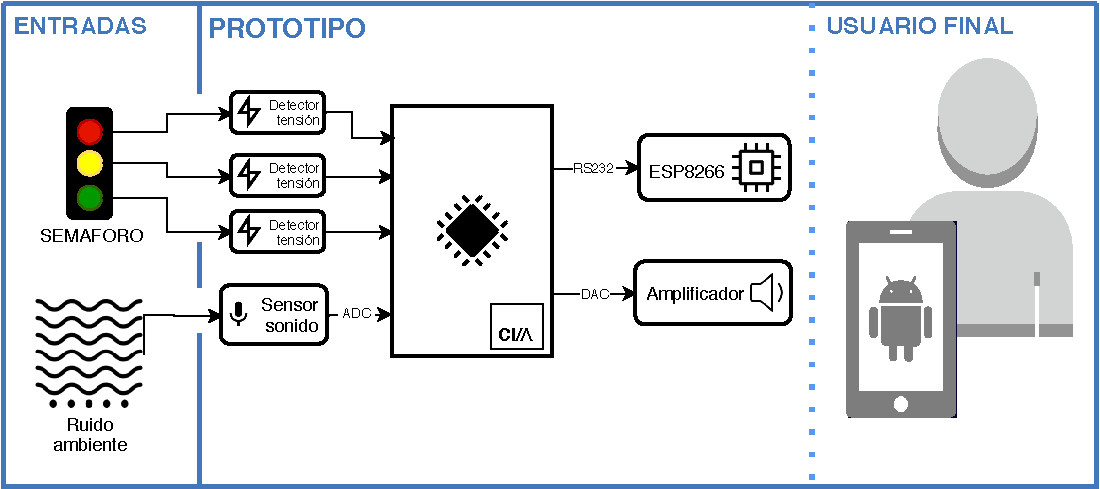
\includegraphics[scale=.7]{./Figures/diagramaGeneralHardware.pdf}
	\caption{Diagrama general del hardware.}
	\label{fig:diagramaGeneralHardware}
\end{figure}

De esta manera se lista los módulos con su respectiva interfaces utilizada:

\begin{itemize}
	\item Detectores de tension: Estos módulos se conectan por los puertos GPIO de la placa.
	\item Sensor de sonido: Se conecta por el puerto analógico digital de la placa.
	\item Amplificador (Salida al parlante): Utiliza el puerto de conversión digital-analógico.
	\item ESP8266: utilizar el otro puerto RS232 que posee la EDU-CIAA.
\end{itemize}

\subsection{Control de volumen}
Un ADC convertidor de señal analógica a digital es un dispositivo electrónico capaz de convertir una señal analógica, ya sea de tensión o corriente, en una señal digital mediante un cuantificador y codificándose en muchos casos en un código binario en particular. Donde un código es la representación unívoca de los elementos, en este caso, cada valor numérico binario hace corresponder a un solo valor de tensión o corriente.

Un conversor de señal digital a analógica o DAC realiza el proceso inverso, es decir, converte señales digitales con datos binarios en señales de corriente o de tensión analógica.

El LPC4737 persente en la EDU-CIAA posee un DAC de 10 bits y dos ADC ambos con una tasa de muestreo maxima de 400 kmuestras por segundo.

La toma de señal se hace a traves de un modulo de sonido por el puerto ADC y la salida de la señal sonora por el puerto DAC. En la siguiente figura \ref{fig:controlVolumen} podemos observar  como es el conexionado a la EDU-CIAA.

\begin{figure}[h]
	\centering
	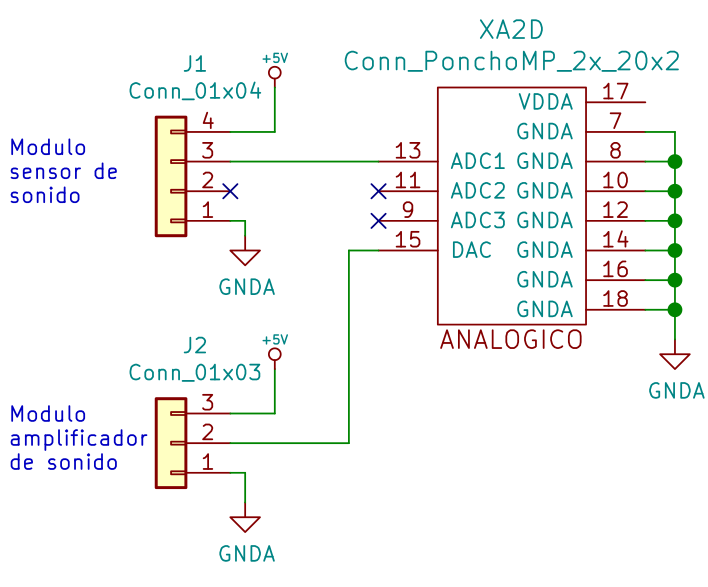
\includegraphics[scale=.3]{./Figures/controlVolumen.png}
	\caption{Conexionado de los modulos. A la derecha las entradas y salidas analogicas de la EDU-CIAA y a la izquierda los pines de conexion para la entrada del modulo de microfono (arriba) y la salida hacia el modulo de amplificacion de sonido (abajo)}
	\label{fig:controlVolumen}
\end{figure}

Segun el nivel de  intensidad del ruido ambiente presente se definio tres tipos de niveles de salida de acuerdo a la entrada. Como se tiene un converson analogico digital de 10 bits quiere decir que el maximo valor  que pude tener es de 1023 con esto se definene los valores en funcion de la entrada.

\begin{itemize}
\item Nivel bajo: 0 a 340
\item Nivel medio: 341 a 680
\item Nivel alto: 681 a 1023
\end{itemize}

\subsection{Dispositivos de comunicación}

En la siguiente figura \ref{fig:conexionESP} se observa el conexionado entre la ESP8266 con la EDU-CIA. La programacion del modulo se hace a traves de comandos AT. Estos tambien conocidos como comandos Hayes es un lenguaje desarrollado por la compañía Hayes Communications que prácticamente se convirtió en estándar abierto de comandos para configurar y parametrizar módems. El envio de los comandos se hacer a traves de la interface RS232 presente en la EDU-CIAA

\begin{figure}[h]
	\centering
	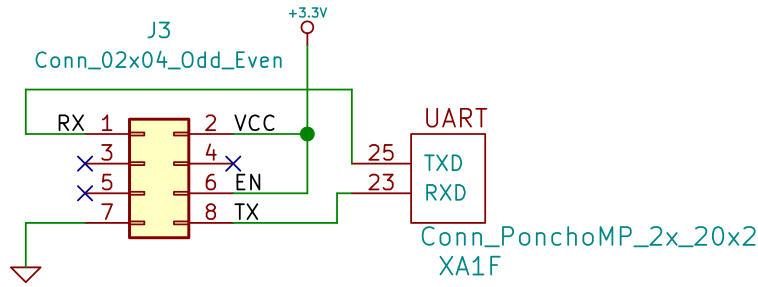
\includegraphics[scale=.5]{./Figures/conexionESP.png}
	\caption{Estructura de capas para el \textit{firmware}.}
	\label{fig:conexionESP}
\end{figure}

\section{Firmware}
\subsection{Arquitectura}
A este proyecto se le dió el nombre de Soniforo, de la conjunción da las palabras sonido y semáforo.

Se optó por un modelo de capas jerárquico para organizar el código en los distintos niveles de abstracción.

En la figura \ref{fig:arquitecturaFirmwareGeneralSistema} se puede observar como se planteó este trabajo. 
\begin{figure}[h]
	\centering
	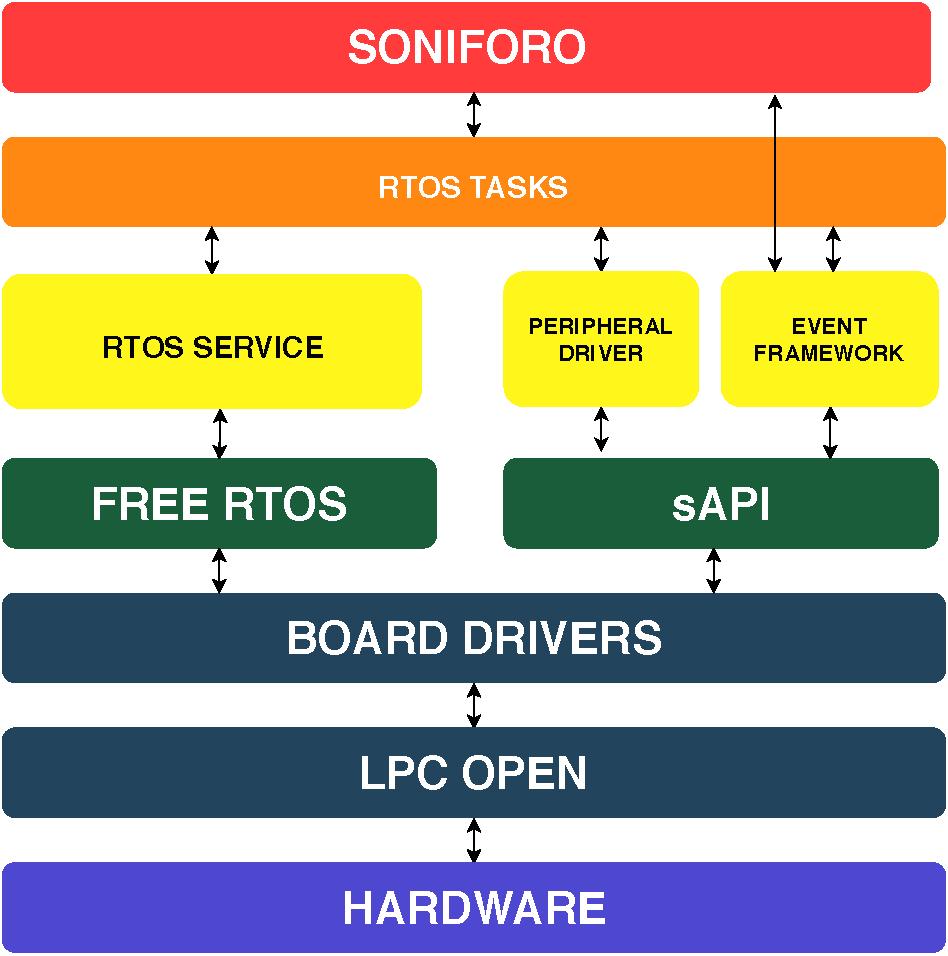
\includegraphics[scale=.5]{./Figures/arquitecturaGeneralSistema.pdf}
	\caption{Estructura de capas para el \textit{firmware}.}
	\label{fig:arquitecturaFirmwareGeneralSistema}
\end{figure}

En cuanto a los niveles de abstracción, la primera capa constituye el hardware de la plataforma EDU-CIAA. La segunda capa, \textit{Hardware Abstraction Layer} (HAL), permite desacoplar las capas superiores del hardware. Aquí se encuentran los
drivers del fabricante del microcontrolador, en el bloque funcional LPC Open. La capa Hardware Independent Layer (HIL) incluye los módulos del RTOS (no está asociada a ningún hardware en particular) y sAPI que permite el manejo de los periféricos de la placa con mayor facilidad.
Sobre esta base se observa una capa orientada a servicio que procesar la información del sistema, estas son: 
\begin{itemize}
\item RTOS Service: Se encarga de la creación de tareas, temporizadores, semáforos binarios.
\item Peripheral Driver: Se encarga de la configuración de los periféricos, como ser las interrupciones.
\item Envent Framework: esta capa se encarga de la definición y creación de todos los eventos del sistema.
\end{itemize}

Sobre estas capas se ubican todas las tareas que corren y son propias del sistema, a esta se la llama RTOS Task. Finalmente, la última capa contiene la aplicación Soniforo.

\subsection{Diseño del firmware}
Para modelar la solución se utilizo una maquina de estado finito, también conocidas como MEF, esta se puede definir como un modelo computacional que realiza cómputos en forma automática sobre una entrada para producir una salida.

Este modelo está conformado por un alfabeto, un conjunto de estados finito, una función de transición, un estado inicial y un conjunto de estados finales.

De esta manera se observa en la siguiente figura \ref{fig:maquinaEstadoFinitoSoniforo}  la maquina de estado finito perteneciente al sistema, por simplicidad algunos estados fueron eliminados para no dificultar el entendimiento (?).

\begin{figure}[h]
	\centering
	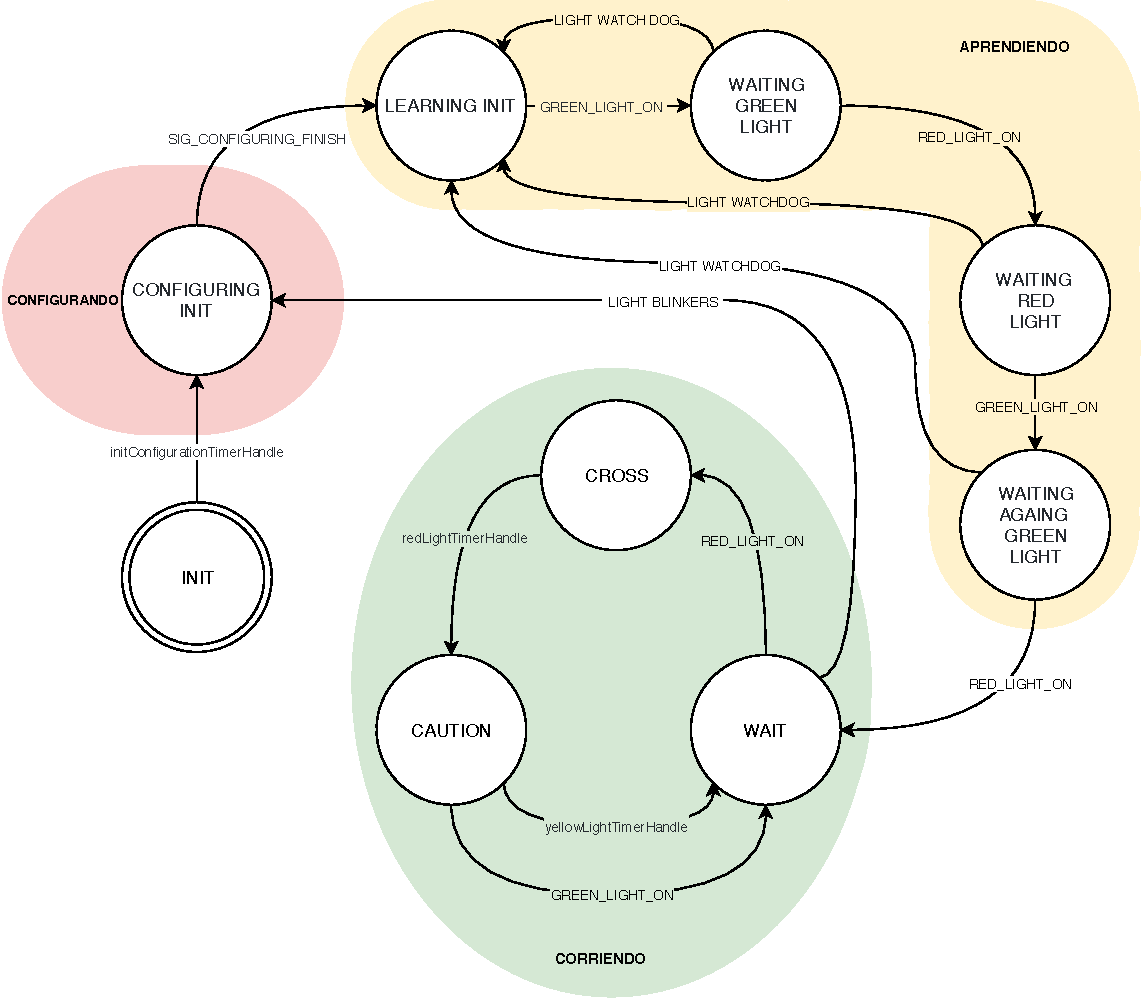
\includegraphics[scale=.7]{./Figures/maquinaEstadoFinitoSoniforo.pdf}
	\caption{Maquina de estado finito del sistema.}
	\label{fig:maquinaEstadoFinitoSoniforo}
\end{figure}

De una manera general el sistema puede encontrarse en 3 estados:

\begin{itemize}
\item Configuracion: Donde se inicializan todos los modulos para la comunicacion con dispositivos externos. 
\item Aprendizaje: El sistema usa el prendido y apagado de las luces del semáforo y con ello aprende su funcionamiento tomando los tiempos de las luces.
\item Corriendo: El sistema funcionando de manera autónoma, siempre y cuando no detecte anomalías en los cambios de las luces del semáforo.
\end{itemize}

\subsubsection{Configuración}
Al energizarse el sistema o luego de un reinicio, el este inicia en el estado INIT donde comienza un temporizador (initConfigurationTimerHandle) que al momento de expirar envía un mensaje para iniciar el sistema, en este momento el sistema pasa a estado CONFIGUING\_INIT este estado consiste en configurar todos los dispositivos de comunicacion externos conectados a la placa principal. 
En el caso particular para la ESP8266 dicha configuración se la hace a traves de comandos AT, lo que se quiere lograr con la esto es que el modulo Wi-Fi levante un punto de acceso inalámbrico, de forma tal que, cualquier teléfono inteligente pueda conectarse a la red inalámbrica propiamente dicha. Tambien una vez configurado correctamente el punto de acceso, se abre una conexion UDP en el puerto 4096 de manera tal que se pueda enviar mensajes broadcast por dicho puerto. (todo: mejorar esta parte)
A continuación se enumeran los comando que debe enviar la EDU-CIAA a traves del puerto RS232 hacia la ESP8266 para poder configurar lo nombrado anteriormente de manera correcta:

\begin{enumerate}
\item{AT}
\item{AT+RST}
\item{AT+CWMODE=2}
\item{AT+CWSAP=``Soniforo\_CIAA'',``'',8,0}
\item{AT+CWDHCP=0,1}
\item{AT+CWDHCP=1,1}
\item{AT+CIPSTART=3,``UDP'',``0'',0,4096,2}
\item{AT+CIPSEND=3,8,``192.168.4.255'',4096}
\item{AT+CIPMUX=1}
\item{AT+CIPDINFO=1}
\item{AT+CWAUTOCONN=0}
\end{enumerate}

Para mas detalle de que hace cada comando el lector puede recurrir a la hoja con comandos que provee el fabricante \citep{esp8266command}.

Cada comando posee una respuesta conocida es por esto que por cada uno enviado se espera la respuesta previamente definida, si esto no sucede después de tres intentos se envía la señal SIG\_FAIL\_CONFIG de manera que el sistema vuelve al estado INIT.

\subsubsection{Aprendizaje}
La solucion abstracta a la problemática radica en cuando un peatón puede o no cruzar la calle.

En argentina no existe un protocolo unico de cambios de luces, por esto para ser indendiente solo se quiere medir el tiempo cuando los autos pasan o esperan por el cambio de luz.

Lo que busca el sistema es tiempo que el peatón pueda cruzar la calle cuando se dispara la luz roja y que tiempo no debe cruzarla,  esto es los tiempos de las luces tanto roja como verde respectivamente, cuando la luz verde del semaforo vehicular se prende signica que el peaton no puede cruzar la calle ya que se encuentran los vehículos en marcha pero cuando la luz cambia a rojo los vehiculos estan detenidos y el peatón puede cruzar la calle.

Como no sabemos a priori en que momento del ciclo el sistema se va a poner en funcionamiento, ni tampoco conocemos que tiempo puede tardar la configuración de los dispositivos de advertencias, el proceso de aprendizaje se hace a traves del encendido u apagado de las luces roja y verde.

Una vez que los dispositivos de advertencia están configurados de manera correcta el sistema pasa al estado LEARNING\_INIT e inmendiatamente se envia al sistema al estado WAITING\_GREEN\_LIGHT  de manera tal que cuando se detecte una luz verde tome el tiempo de inicio, envia el mensjae de poner al sistema en estado WAITING\_RED\_LIGHT cuando llega la luz roja se detiene el tiempo de la luz verde e inicializa el tiempo para la luz roja mientras espera nueva mente la luz ver, es por esto que se envia una mensaje para pasar al sistema al estado WAITING\_AGAIN\_GREEN\_LIGHT. 

Graficamente podemos ejemplificar la secuencia con un ejemplo.

Se puede observar en la figura  \ref{fig:digramaGraficoCambioSemaforo} para el caso donde la secuencia de las luces son rojo, rojo-amarillo, verde, amarillo, rojo.
Tomando como base que el sistema termino de configurarse correctamente cuando el semáforo estaba en luz roja.

\begin{figure}[h]
	\centering
	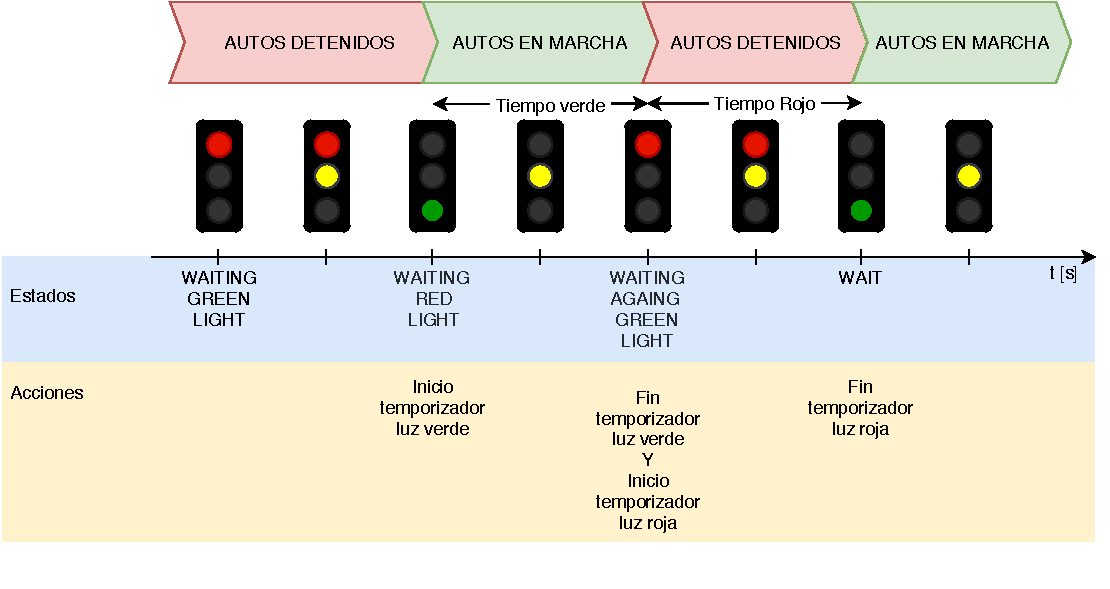
\includegraphics[scale=.7]{./Figures/digramaGraficoCambioSemaforo.pdf}
	\caption{Maquina de estado finito del sistema.}
	\label{fig:digramaGraficoCambioSemaforo}
\end{figure}

Si por alguna razón se detecta alguna anomalia, como ser un semaforo fuera de servicio el sistema regresa al estado LEARNING INIT. Esto se logra atravez de un temporizador que debe actualizarce cada 65 segundos, si esto no acurre se ejecuta la accion definida anteriormente.

\subsubsection{Corriendo}
Una vez finalizado correctamente el aprendizaje de los tiempos, el sistema calcula el tiempo limite para indicar a la persona que puede cruzar la calle tranquilamente, esto se hace a traves de la siguiente formula \ref{eq:calculoTiempoAmarillo}.

esto se implemento de esta forma porque 

\begin{equation}
\label{eq:calculoTiempoAmarillo}
yellowLightTimerHandle = tiempoLuzRojo * 0.35
\end{equation}

De igual manera se hace el calculo para el temporizador de luz roja  formula \ref{eq:calculoTiempoRojo}

\begin{equation}
\label{eq:calculoTiempoRojo}
redLightTimerHandle = tiempoLuzRojo * 0.35
\end{equation}

Estos porcentajes fueron calculados de manera empirica. (decir algo mas) 
Estos temporizadores son gestionado por el FreeRTOS de manera tal que cuando expiren llamen a funciones predefinidas en el momento de la creacion de estos.

El sistema posee tres temporizadores los cuales son iniciados cuando se detecta una luz encendida.

\begin{itemize}
\item redLightTimerHandle: tiempo de la luz roja encendida.
\item yellowLightTimerHandle: se mide en base a la luz roja como se menciono anteriormente.
\item greenLightTimerHandle: tiempo de la luz verde.
\end{itemize}

Una vez configurados los temporizadores, se espera una interrupción de la luz roja para desbloquear la tarea de enviar el estado CROSS a la ESP8266 y ademas empieza a correr el temporizador de la luz roja, cuando este expira se bloquea la tarea de enviar el estado de CROSS y se desbloquea la tarea de enviar el estado CAUTION y se incializa el temporizador de la luz amarilla, cabe recordar como se mensiono que los mensajes broadcast UDP  a traves del puerto 4096. Una vez que vence este temporizador se bloque la tarea de enviar el estado CROSS y se espera nuevamente por la señal de la luz roja encendida.

\section{Principio de funcionamiento}
El firmware fue diseñado en base a distintos patrones de software vistos a lo largo de la carrera, principalmente el sistema se basa en el diseño Observar y reaccionar, este patron nos permite reaccionar a distintos eventos y reaccionar de una manera predefinida en conjunto con este patron el sistema implementa Lazos de eventos. Donde las reacciones produce mensajes y segun el estado en el cual este el sistema dispara alguna accion. Donde en nuestro caso particular estas reacciones generan transiciones de estados.

En la figura \ref{fig:generalWorkFlow} se puede observar el flujo de trabajo del sistema, donde los eventos que produce el semaforo se envian a una cola que segun el tipo de evento y el estado del sistema reacciona de una manera definida.

\begin{figure}[H]
	\centering
	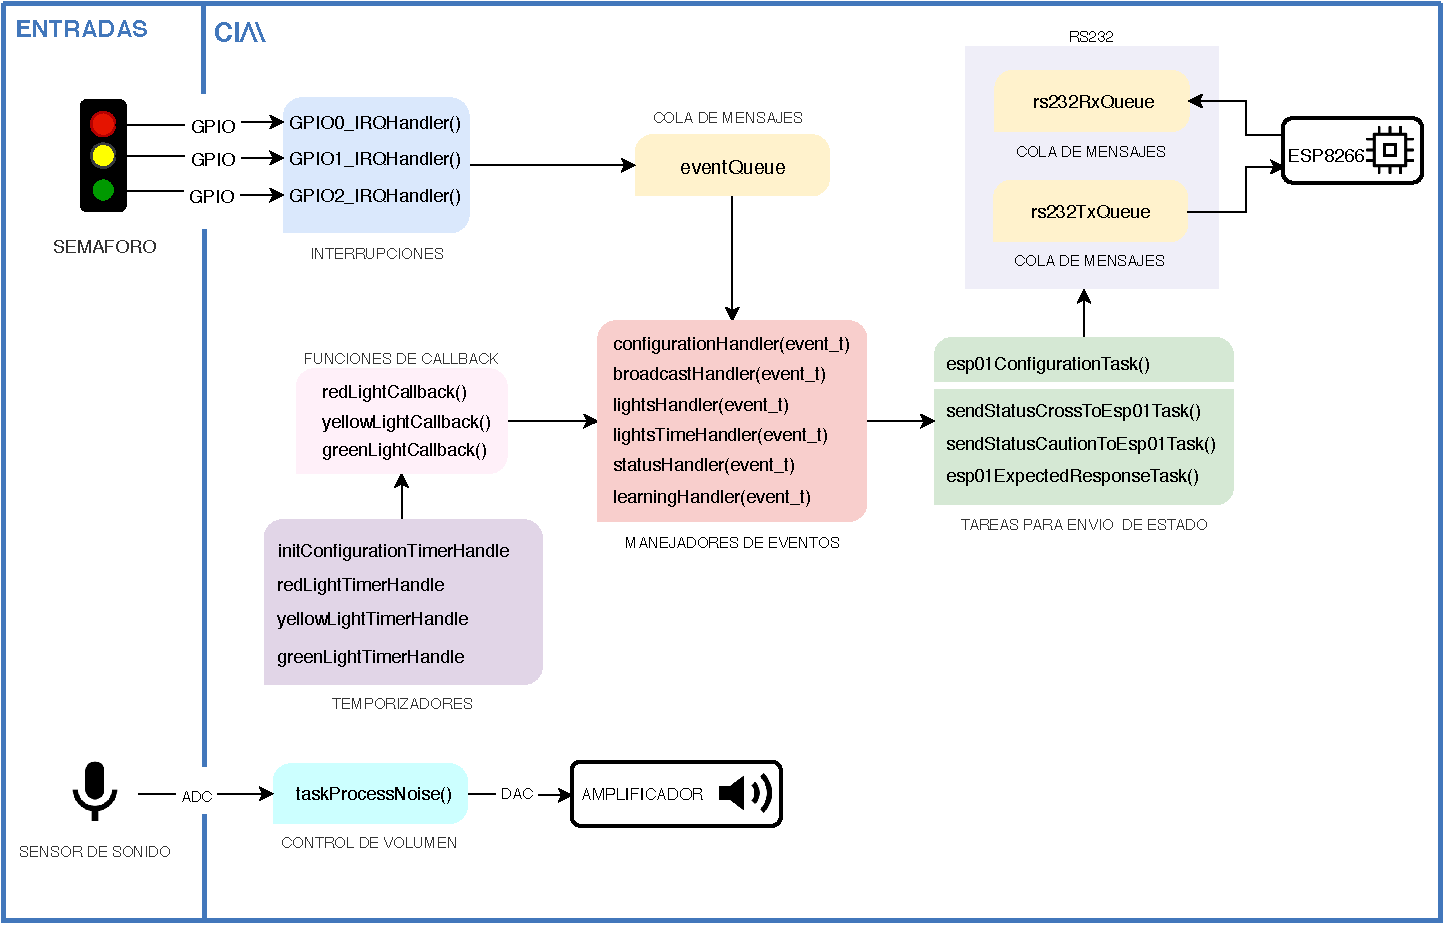
\includegraphics[scale=.6]{./Figures/generalWorkFlow.pdf}
	\caption{Diagrama general de funcionamiento.}
	\label{fig:generalWorkFlow}
\end{figure}

Es por eso que se define un tipo de dato especial para enviar el evento hacia una cola.

\lstset{language=C, breaklines=true, basicstyle=\footnotesize}
\begin{lstlisting}
struct event_t {
	module_t * receptor;
	int signal;
	led_name_t ledName;
};
\end{lstlisting}

Los tipos de estados de las luces pueden ser:

\begin{itemize}
\item Luz encendida
\item Luz Apagada
\end{itemize}

(No se si poner este ejemplo)
Podemo ejemplicar este flujo con un ejemplo, en el caso en el cual prenden la luz roja seria:
\begin{enumerate}
\item Se produce una interrupción de la luz roja.
\item Esta interrupcion es manejada por su funcion.
\item Se envia un evento a la cola eventQueue
\item La tarea encargada de recibir los eventos, lee el mensaje y ejecuta el manejador correspondiente.
\item Se ejecuta la accion
\end{enumerate}

\section{Aplicacion android}
Para poder recibir los estados del semaforo correctamente se diseño una aplicacion muy simple para la plataforma movil android, esta corre desdeAndroid 4.0.0 (Ice Cream Sandwich) \citep{androidVersion}, dicha aplicación es capaz de vibrar según el tipo de comando que reciba desde el prototipo. En la siguiente tabla \ref{tab:vibraciones} se muestra la relación entre los estados enviados y el tipo de vibración que produce.

\begin{table}[h]
\centering
\caption[caption corto]{Relación entre el estado del semáforo y las vibraciones emitidas}
\begin{tabular}{l c}
\toprule
\textbf{Estado enviado} & \textbf{Tipo de vibraciones}\\
\midrule
Esperar & Sin vibraciones\\
Cruzar &  Vibraciones 2 segundo con 2 segundo de espera\\
Precaucion & Vibraciones de 1 segundo con 1 segundo de espera\\
\bottomrule
\hline
\end{tabular}
\label{tab:vibraciones}
\end{table}

La aplicación móvil tiene una interface muy simple y esta orientada a la correcta visualización de los estados del semáforo. Como se puede observar en la figura \ref{fig:androidApplication} posee dos botones, uno para conectar al servidor broadcast en el puerto 4096 y otro para detener la conexión, edemas posee  una pantalla donde se pueden visualizar los mensajes enviados desde Soniforo.

\begin{figure}[h]
	\centering
	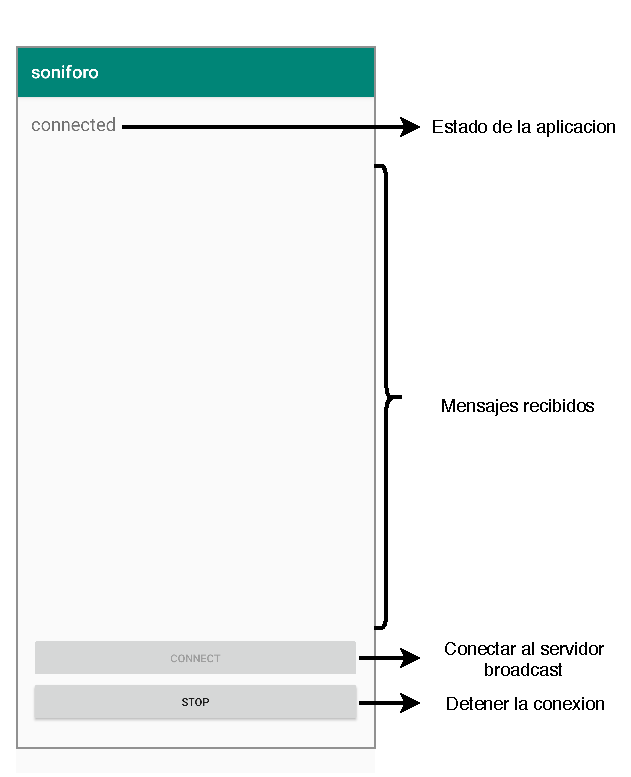
\includegraphics[scale=.5]{./Figures/androidApplication.pdf}
	\caption{Interface grafica de la aplicacion android desarrollada}
	\label{fig:androidApplication}
\end{figure}

\section{Poncho}
Para poder conectar los modulos externos principal EDU-CIA se utilizó la aplicación Eeschema del KiCAD 5. El diseño se llevó a cabo conectando los puertos de expansión -o interfaz- de la EDU-CIAA-NXP a los diferentes modulos externos, tambien adicionalmente se agrego puertos para conectar una fuente externar de manera tal que la placa princial  no tenga exigencia de corrientes. 
(Habria que poner que se hizo un calculo de las corriente que sacan lo perifericos)
Se puede observar en la siguiente figura el equema general de conexionado

\section{Gabinete}